\documentclass[border=6pt]{standalone}
\usepackage{times}
\usepackage{pgfplots}
\pgfplotsset{compat=1.18}
\begin{document}
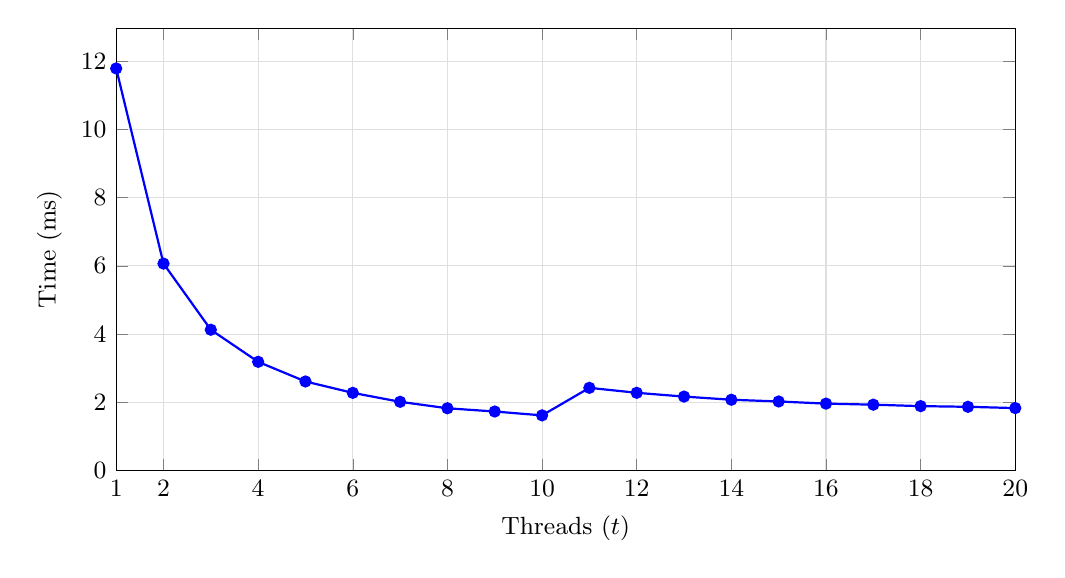
\begin{tikzpicture}
\begin{axis}[width=13cm,height=7.2cm,
xlabel={Threads ($t$)},ylabel={Time (ms)},
xmin=1,xmax=20,xtick={1,2,4,6,8,10,12,14,16,18,20},
ymin=0,grid=both,major grid style={gray!25},minor grid style={gray!10},
tick label style={font=\small},label style={font=\small},
scaled y ticks=false,/pgf/number format/1000 sep={}]
\addplot[blue,thick,mark=*,mark size=1.8pt] coordinates {
(1, 11.783552)
(2, 6.065859)
(3, 4.12759)
(4, 3.187407)
(5, 2.611829)
(6, 2.278323)
(7, 2.01604)
(8, 1.827026)
(9, 1.731696)
(10, 1.618834)
(11, 2.425656)
(12, 2.280163)
(13, 2.169242)
(14, 2.07684)
(15, 2.025849)
(16, 1.963159)
(17, 1.932248)
(18, 1.889358)
(19, 1.869858)
(20, 1.832307)
};
\end{axis}
\end{tikzpicture}
\end{document}
